\documentclass[11pt,a4paper,ja=standard]{ltjsarticle}
\usepackage{amsmath,amssymb,amsthm}
\usepackage{mathtools}
\usepackage{tikz}
\usetikzlibrary{cd,arrows,positioning}
\usepackage{geometry}
\geometry{margin=2.5cm}
\usepackage{hyperref}
\usepackage{enumitem}
\usepackage{url}

% 定理環境
\theoremstyle{definition}
\newtheorem{definition}{定義}[section]
\newtheorem{theorem}[definition]{定理}
\newtheorem{lemma}[definition]{補題}
\newtheorem{proposition}[definition]{命題}
\newtheorem{corollary}[definition]{系}
\newtheorem{example}[definition]{例}
\newtheorem{remark}[definition]{注意}

% コマンド定義
\newcommand{\N}{\mathbb{N}}
\newcommand{\R}{\mathbb{R}}
\newcommand{\F}{\mathcal{F}}
\newcommand{\G}{\mathcal{G}}
\newcommand{\minLayer}{\mathrm{minLayer}}
\newcommand{\layer}{\mathrm{layer}}

\title{構造塔理論による停止時間の形式化}
\author{Claude Code (Anthropic) \and CODEX (OpenAI)\thanks{%
本論文のLean 4形式化コードはClaude CodeおよびCODEX (OpenAI)により生成された。}}
\date{\today}

\begin{document}

\maketitle

\begin{abstract}
本章では、構造塔（structure tower）のフレームワークを用いて、確率論における停止時間（stopping time）の理論を統一的に形式化する。
従来の確率論では、フィルトレーション、停止時間、停止 $\sigma$-代数、停止過程などの概念が個別に導入されていたが、
構造塔の観点からは、これらすべてが「階層的包含構造」の特殊ケースとして統一的に扱えることを示す。
特に、Bourbaki的な母構造の視点に立ち、$\sigma$-代数の族を順序構造として捉え直すことで、
測度論や期待値に依存せずに停止時間の基本性質を導出する。
本章の形式化はLean 4で実装され、\texttt{sorry}なしで検証可能である。
\end{abstract}

\tableofcontents

\section{導入}

\subsection{背景と動機}

確率論における停止時間の理論は、マルチンゲール理論の中核をなす重要な概念である。
しかし、教科書的な定義では、停止時間 $\tau$ に対する「停止 $\sigma$-代数 $\F_\tau$」や
「停止過程 $X^\tau$」の構成が、場当たり的な集合演算の組み合わせとして提示されることが多く、
背後にある統一的な構造が見えにくい。

本章では、Bourbakiの構造概念を現代的に再解釈した「構造塔（structure tower）」の枠組みを用いることで、
停止時間に関するすべての構成が、以下の単純な原理に基づくことを明らかにする：

\begin{center}
\fbox{%
\parbox{0.9\textwidth}{%
\textbf{構造塔の原理}：
数学的構造の階層的包含関係 $S_0 \subseteq S_1 \subseteq S_2 \subseteq \cdots$ は、
各点がいつ初めて構造に入るかを記述する「最小層関数 $\minLayer$」によって完全に特徴づけられる。
}%
}
\end{center}

この原理の下では、フィルトレーション $(\F_n)_{n \in \N}$ は $\sigma$-代数の塔であり、
停止時間 $\tau$ は「各点 $\{\omega\}$ が初めて可測になる時刻」として定義され、
停止 $\sigma$-代数 $\F_\tau$ は「切り詰め停止時間 $\tau \wedge n$ の塔」として自動的に構成される。

\subsection{本章の構成}

\begin{itemize}[leftmargin=*]
\item \textbf{第2節}：構造塔と $\minLayer$ の一般論（概観）
\item \textbf{第3節}：$\sigma$-代数とフィルトレーションを構造塔として定式化
\item \textbf{第4節}：停止時間の定義と基本性質
\item \textbf{第5節}：停止 $\sigma$-代数の構成
\item \textbf{第6節}：停止フィルトレーションの核（$\mathtt{covers}$を仮定しない形）
\item \textbf{第7節}：停止過程と停止前後の振る舞い
\item \textbf{第8節}：まとめと展望
\end{itemize}

\section{構造塔と $\minLayer$ の一般論}

\subsection{構造塔の定義}

構造塔は、ある型 $X$ 上の構造の族 $S: I \to \mathcal{P}(X)$（$I$ は全順序集合）が満たすべき性質を抽象化したものである。

\begin{definition}[構造塔の最小骨格]\label{def:structure-tower-min}
型 $X$ と全順序インデックス集合 $I$ に対し、\emph{構造塔 $\mathtt{StructureTowerMin}(X, I)$} は以下のデータからなる：
\begin{enumerate}[label=(\roman*)]
\item \textbf{層関数}：$\layer : I \to \mathcal{P}(X)$
\item \textbf{単調性}：$i \le j \implies \layer(i) \subseteq \layer(j)$
\item \textbf{最小層関数}：$\minLayer : X \to I$
\item \textbf{最小層の所属}：$\forall x \in X,\ x \in \layer(\minLayer(x))$
\item \textbf{最小性}：$\forall x \in X,\ \forall i \in I,\ (x \in \layer(i) \implies \minLayer(x) \le i)$
\end{enumerate}
\end{definition}

\begin{remark}
定義\ref{def:structure-tower-min}は、測度論的な仮定（測度空間、可測性など）を一切含まない純粋な順序構造である。
これにより、位相空間の開集合族、環のイデアル包含、群の部分群連鎖など、
多様な数学的構造を統一的に扱うことができる。
\end{remark}

\subsection{構造塔の図式表現}

構造塔の本質は、次の可換図式で表される：

\begin{center}
\begin{tikzpicture}[node distance=2.5cm, auto]
  \node (X) {$X$};
  \node (I) [right of=X] {$I$};
  \node (PX) [below of=X] {$\mathcal{P}(X)$};

  \draw[->] (X) -- node {$\minLayer$} (I);
  \draw[->] (I) -- node[swap] {$\layer$} (PX);
  \draw[->] (X) -- node[swap] {$x \mapsto \{x\}$} (PX);

  \node at (1.2,-1.5) {\small 最小性};
\end{tikzpicture}
\end{center}

各点 $x \in X$ は、$\minLayer(x)$ で初めて $\layer$ に入り、それ以降すべての層に含まれる。

\section{$\sigma$-代数とフィルトレーションの構造塔表現}

\subsection{フィルトレーションの定義}

確率空間 $(\Omega, \F)$ 上のフィルトレーションは、増大する $\sigma$-代数の族である。

\begin{definition}[フィルトレーション]\label{def:filtration}
可測空間 $(\Omega, \F)$ 上の\emph{フィルトレーション} $(\F_n)_{n \in \N}$ とは、
以下を満たす $\sigma$-代数の族である：
\begin{enumerate}[label=(\roman*)]
\item $\F_n$ は $\Omega$ 上の $\sigma$-代数
\item $n \le m \implies \F_n \subseteq \F_m$（単調性）
\end{enumerate}
\end{definition}

\begin{remark}
本章では、さらに「各 $\F_n$ が $\Omega$ 全体を生成する」という $\mathtt{covers}$ 条件を課すことで、
$\minLayer$ が well-defined になることを保証する。
ただし、停止フィルトレーションの構成では $\mathtt{covers}$ を要求しない
「フィルトレーション核（$\mathtt{SigmaAlgebraFiltration.Core}$）」も導入する。
\end{remark}

\subsection{フィルトレーションから構造塔への昇格}

フィルトレーション $\F = (\F_n)$ は、次の対応により構造塔を誘導する：

\begin{proposition}[フィルトレーションの塔化]\label{prop:filtration-to-tower}
フィルトレーション $\F = (\F_n)_{n \in \N}$ に対し、
\[
\mathtt{towerOf}(\F) := \mathtt{StructureTowerMin}(\mathcal{P}(\Omega), \N)
\]
を次のように定義する：
\begin{align*}
\layer(n) &:= \{ A \subseteq \Omega \mid A \in \F_n \} \\
\minLayer(A) &:= \min \{ n \in \N \mid A \in \F_n \}
\end{align*}
このとき、$\mathtt{towerOf}(\F)$ は定義\ref{def:structure-tower-min}を満たす。
\end{proposition}

\begin{proof}
単調性は $\F_n \subseteq \F_m$ から直ちに従う。
$\mathtt{covers}$ 条件により、任意の単点 $\{\omega\}$ に対し $\{\omega\} \in \F_n$ となる $n$ が存在するため、
$\minLayer(\{\omega\})$ が well-defined である。最小性は $\min$ の定義から明らか。
\end{proof}

\subsection{構造塔の図式：フィルトレーションの場合}

\begin{center}
\begin{tikzpicture}[>=stealth, node distance=3cm, auto]
  % Top row
  \node (F0) {$\F_0$};
  \node (F1) [right of=F0] {$\F_1$};
  \node (F2) [right of=F1] {$\F_2$};
  \node (dots) [right of=F2] {$\cdots$};

  % Arrows
  \draw[right hook->] (F0) -- (F1);
  \draw[right hook->] (F1) -- (F2);
  \draw[right hook->] (F2) -- (dots);

  % Labels
  \node at (1.5, -0.7) {\small 単調包含};

  % Bottom: minLayer
  \node (omega) at (0, -2) {$\omega \in \Omega$};
  \node (arrow) at (0, -3) {};
  \draw[->] (omega) -- node[left] {\small $\minLayer(\{\omega\})$} (arrow);
  \node at (0, -3.5) {\small 初めて $\{\omega\}$ が可測になる時刻};
\end{tikzpicture}
\end{center}

\section{停止時間の定義と基本性質}

\subsection{古典的な停止時間}

\begin{definition}[停止時間]\label{def:stopping-time}
フィルトレーション $\F = (\F_n)_{n \in \N}$ に対し、
$\Omega \to \N$ なる関数 $\tau$ が\emph{停止時間}であるとは、
\[
\forall n \in \N,\quad \{\omega \in \Omega \mid \tau(\omega) \le n\} \in \F_n
\]
が成り立つことをいう。
\end{definition}

\begin{remark}
集合 $\{\tau \le n\}$ は「時刻 $n$ までに停止が起こったか否か」を $\F_n$ の情報だけで判定できることを意味する。
これが停止時間の「適合性（adaptedness）」の本質である。
\end{remark}

\subsection{停止集合と構造塔の層}

\begin{lemma}[停止集合の塔所属性]\label{lem:stopping-sets-in-tower}
停止時間 $\tau$ に対し、任意の $n \in \N$ について
\[
\{\omega \mid \tau(\omega) \le n\} \in \layer(n)
\]
が成り立つ。すなわち、停止集合は構造塔の第 $n$ 層に属する。
\end{lemma}

\begin{proof}
定義\ref{def:stopping-time}より $\{\tau \le n\} \in \F_n$ であり、
命題\ref{prop:filtration-to-tower}より $\F_n = \layer(n)$ だから明らか。
\end{proof}

\subsection{最小可測時刻}

構造塔の $\minLayer$ を用いて、各点が初めて可測になる時刻を定義できる。

\begin{definition}[最初の可測時刻]\label{def:first-measurable-time}
フィルトレーション $\F$ と点 $\omega \in \Omega$ に対し、
\[
\mathtt{firstMeasurableTime}(\F, \omega) := \minLayer_{\mathtt{towerOf}(\F)}(\{\omega\})
\]
を $\omega$ の\emph{最初の可測時刻}という。
\end{definition}

\begin{theorem}[単点の可測性]\label{thm:singleton-measurable}
任意の $\omega \in \Omega$ に対し、
\[
\{\omega\} \in \F_{\mathtt{firstMeasurableTime}(\F, \omega)}
\]
が成り立ち、かつこれは可測となる最小の時刻である。
\end{theorem}

\begin{proof}
構造塔の $\minLayer$ の所属性と最小性（定義\ref{def:structure-tower-min}）から直ちに従う。
\end{proof}

\section{停止 $\sigma$-代数の構成}

\subsection{停止 $\sigma$-代数の定義}

停止 $\sigma$-代数は、「時刻 $\tau$ までの情報」を表す $\sigma$-代数である。

\begin{definition}[停止 $\sigma$-代数]\label{def:stopped-sigma-algebra}
フィルトレーション $\F$ と停止時間 $\tau$ に対し、
\emph{停止 $\sigma$-代数 $\F_\tau$} を次で定義する：
\[
A \in \F_\tau \quad \Longleftrightarrow \quad
\forall n \in \N,\ A \cap \{\tau \le n\} \in \F_n
\]
\end{definition}

\begin{remark}
この定義は「$A$ が $\F_\tau$ に属する」ことを、
「各時刻 $n$ で観測される $A$ の部分（$A \cap \{\tau \le n\}$）が $\F_n$-可測」
という条件で特徴づけている。
\end{remark}

\subsection{停止 $\sigma$-代数の図式}

\begin{center}
\begin{tikzpicture}[>=stealth, node distance=2.5cm]
  % Left: original filtration
  \node (F0) at (0, 2) {$\F_0$};
  \node (F1) at (0, 1) {$\F_1$};
  \node (F2) at (0, 0) {$\F_2$};
  \node (dots1) at (0, -0.8) {$\vdots$};

  \draw[right hook->] (F0) -- (F1);
  \draw[right hook->] (F1) -- (F2);

  % Right: stopped filtration
  \node (Ft0) at (4, 2) {$\F_{\tau \wedge 0}$};
  \node (Ft1) at (4, 1) {$\F_{\tau \wedge 1}$};
  \node (Ft2) at (4, 0) {$\F_{\tau \wedge 2}$};
  \node (dots2) at (4, -0.8) {$\vdots$};
  \node (Ftau) at (4, -1.5) {$\F_\tau$};

  \draw[right hook->] (Ft0) -- (Ft1);
  \draw[right hook->] (Ft1) -- (Ft2);
  \draw[->] (dots2) -- (Ftau);

  % Horizontal arrows
  \draw[->] (F0) -- node[above] {\small 切り詰め} (Ft0);
  \draw[->] (F1) -- (Ft1);
  \draw[->] (F2) -- (Ft2);

  \node at (2, -2.3) {$\F_\tau = \sup_{n} \F_{\tau \wedge n}$};
\end{tikzpicture}
\end{center}

\subsection{停止 $\sigma$-代数の基本性質}

\begin{lemma}[停止集合の所属性]\label{lem:stopping-set-in-stopped}
任意の $n \in \N$ に対し、
\[
\{\tau \le n\} \in \F_\tau
\]
が成り立つ。
\end{lemma}

\begin{proof}
任意の $k \in \N$ に対し、
\[
\{\tau \le n\} \cap \{\tau \le k\} = \{\tau \le \min(n, k)\} \in \F_{\min(n,k)} \subseteq \F_k
\]
となるため、定義\ref{def:stopped-sigma-algebra}を満たす。
\end{proof}

\begin{theorem}[停止時間の大小と $\sigma$-代数の包含]\label{thm:stopped-sigma-monotone}
$\tau_1, \tau_2$ を停止時間とし、$\tau_1(\omega) \le \tau_2(\omega)$ が任意の $\omega$ で成り立つならば、
\[
\F_{\tau_1} \subseteq \F_{\tau_2}
\]
が成り立つ。
\end{theorem}

\begin{proof}
$A \in \F_{\tau_1}$ とすると、任意の $n$ に対し $A \cap \{\tau_1 \le n\} \in \F_n$。
$\tau_1 \le \tau_2$ より $\{\tau_2 \le n\} \subseteq \{\tau_1 \le n\}$ なので、
\[
A \cap \{\tau_2 \le n\} = (A \cap \{\tau_1 \le n\}) \cap \{\tau_2 \le n\} \in \F_n
\]
となり、$A \in \F_{\tau_2}$ を得る。
\end{proof}

\section{停止フィルトレーションの核}

\subsection{切り詰め停止時間}

\begin{definition}[切り詰め停止時間]\label{def:truncate-stopping-time}
停止時間 $\tau$ と $n \in \N$ に対し、
\[
(\tau \wedge n)(\omega) := \min(\tau(\omega), n)
\]
を\emph{切り詰め停止時間}という。
\end{definition}

\begin{lemma}[切り詰めの単調性]\label{lem:truncate-monotone}
$n \le m$ ならば、任意の $\omega$ に対し
\[
(\tau \wedge n)(\omega) \le (\tau \wedge m)(\omega)
\]
が成り立つ。
\end{lemma}

\begin{proof}
$\min(\tau(\omega), n) \le \min(\tau(\omega), m)$ は $n \le m$ から直ちに従う。
\end{proof}

\subsection{停止フィルトレーション核の定義}

\begin{definition}[停止フィルトレーション核]\label{def:stopped-filtration-core}
停止時間 $\tau$ に対し、\emph{停止フィルトレーション核 $\G_\tau$} を
\[
\G_\tau := (\F_{\tau \wedge n})_{n \in \N}
\]
で定義する。ただし、$\F_{\tau \wedge n}$ は定義\ref{def:stopped-sigma-algebra}による停止 $\sigma$-代数である。
\end{definition}

\begin{remark}
「核（core）」と呼ぶのは、$\mathtt{covers}$ 条件を満たさない可能性があるためである。
すなわち、$\bigcup_n \F_{\tau \wedge n}$ が $\Omega$ 全体を生成するとは限らない。
しかし、単調性 $\G_\tau(n) \subseteq \G_\tau(m)$ for $n \le m$ は補題\ref{lem:truncate-monotone}と定理\ref{thm:stopped-sigma-monotone}から保証される。
\end{remark}

\subsection{停止フィルトレーション核の図式}

\begin{center}
\begin{tikzpicture}[>=stealth, node distance=2cm, auto]
  % Original process at top
  \node (X0) at (0, 3) {$\F_0$};
  \node (X1) at (1.5, 3) {$\F_1$};
  \node (X2) at (3, 3) {$\F_2$};
  \node (Xdots) at (4.5, 3) {$\cdots$};

  \draw[right hook->] (X0) -- (X1);
  \draw[right hook->] (X1) -- (X2);
  \draw[right hook->] (X2) -- (Xdots);

  \node at (-1, 3) {\small 元の $\F$:};

  % Stopped filtration core below
  \node (G0) at (0, 1) {$\F_{\tau \wedge 0}$};
  \node (G1) at (1.5, 1) {$\F_{\tau \wedge 1}$};
  \node (G2) at (3, 1) {$\F_{\tau \wedge 2}$};
  \node (Gdots) at (4.5, 1) {$\cdots$};

  \draw[right hook->] (G0) -- (G1);
  \draw[right hook->] (G1) -- (G2);
  \draw[right hook->] (G2) -- (Gdots);

  \node at (-1, 1) {\small $\G_\tau$:};

  % Vertical arrows
  \draw[->] (X0) -- (G0);
  \draw[->] (X1) -- (G1);
  \draw[->] (X2) -- (G2);

  \node at (6, 2) {包含関係};
  \draw[right hook->] (5.5, 1.8) -- (5.5, 2.2);
\end{tikzpicture}
\end{center}

\subsection{停止フィルトレーション核の基本性質}

\begin{proposition}[停止フィルトレーションと元のフィルトレーションの関係]\label{prop:stopped-filtration-le}
任意の $n \in \N$ に対し、
\[
\F_{\tau \wedge n} \subseteq \F_n
\]
が成り立つ。
\end{proposition}

\begin{proof}
$A \in \F_{\tau \wedge n}$ とすると、定義より任意の $k$ に対し
\[
A \cap \{(\tau \wedge n) \le k\} \in \F_k
\]
が成り立つ。特に $k = n$ とすると、
\[
\{(\tau \wedge n) \le n\} = \Omega
\]
なので、$A \cap \Omega = A \in \F_n$ を得る。
\end{proof}

\begin{lemma}[停止集合の可測性（停止フィルトレーション核内）]\label{lem:stopping-set-in-core}
任意の $n \in \N$ に対し、
\[
\{\tau \le n\} \in \F_{\tau \wedge n}
\]
が成り立つ。
\end{lemma}

\begin{proof}
任意の $k \in \N$ に対し、
\begin{align*}
\{\tau \le n\} \cap \{(\tau \wedge n) \le k\}
&= \begin{cases}
\{\tau \le k\} & \text{if } k < n \\
\{\tau \le n\} & \text{if } k \ge n
\end{cases}
\end{align*}
となり、いずれも $\F_k$ に属する（$\tau$ が停止時間であることから）。
\end{proof}

\section{停止過程と停止前後の振る舞い}

\subsection{停止過程の定義}

\begin{definition}[停止過程]\label{def:stopped-process}
確率過程 $X = (X_n)_{n \in \N}$ と停止時間 $\tau$ に対し、
\emph{停止過程 $X^\tau$} を
\[
X^\tau_n(\omega) := X_{\min(n, \tau(\omega))}(\omega)
\]
で定義する。
\end{definition}

\begin{remark}
停止過程は、「停止時刻 $\tau(\omega)$ に達したら、その値で固定される」過程である。
これはオプショナル停止定理の鍵となる構成である。
\end{remark}

\subsection{停止過程の図式}

\begin{center}
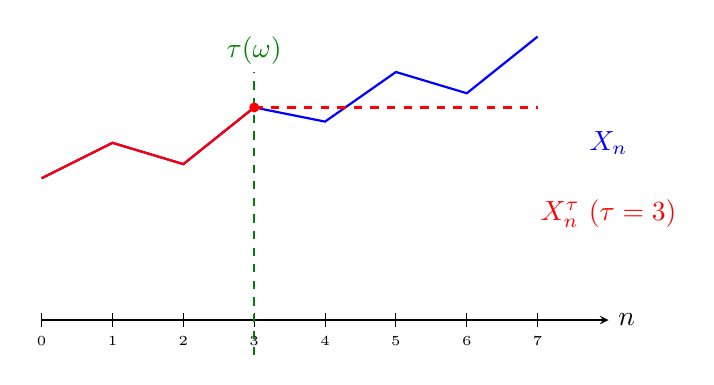
\begin{tikzpicture}[>=stealth, scale=0.9]
  % Time axis
  \draw[->] (0,0) -- (8,0) node[right] {$n$};
  \foreach \x in {0,1,2,3,4,5,6,7}
    \draw (\x, 0.1) -- (\x, -0.1) node[below] {\tiny $\x$};

  % Original process X
  \draw[thick, blue] (0,2) -- (1,2.5) -- (2,2.2) -- (3,3) -- (4,2.8) -- (5,3.5) -- (6,3.2) -- (7,4);
  \node at (8, 2.5) [blue] {$X_n$};

  % Stopped process X^tau (tau = 3)
  \draw[thick, red] (0,2) -- (1,2.5) -- (2,2.2) -- (3,3);
  \draw[thick, red, dashed] (3,3) -- (4,3) -- (5,3) -- (6,3) -- (7,3);
  \node at (8, 1.5) [red] {$X^\tau_n$ ($\tau = 3$)};

  % Stopping time marker
  \draw[thick, green!50!black, dashed] (3, -0.5) -- (3, 3.5);
  \node at (3, 3.8) [green!50!black] {$\tau(\omega)$};

  \fill[red] (3,3) circle (2pt);
\end{tikzpicture}
\end{center}

\subsection{停止過程の基本性質}

\begin{theorem}[停止前では元の過程と一致]\label{thm:stopped-eq-before}
$n \le \tau(\omega)$ ならば、
\[
X^\tau_n(\omega) = X_n(\omega)
\]
が成り立つ。
\end{theorem}

\begin{proof}
$\min(n, \tau(\omega)) = n$ なので、定義\ref{def:stopped-process}より明らか。
\end{proof}

\begin{theorem}[停止後は値が固定される]\label{thm:stopped-const-after}
$\tau(\omega) \le n \le m$ ならば、
\[
X^\tau_m(\omega) = X^\tau_n(\omega)
\]
が成り立つ。
\end{theorem}

\begin{proof}
\begin{align*}
X^\tau_m(\omega) &= X_{\min(m, \tau(\omega))}(\omega) = X_{\tau(\omega)}(\omega) \\
X^\tau_n(\omega) &= X_{\min(n, \tau(\omega))}(\omega) = X_{\tau(\omega)}(\omega)
\end{align*}
となるため、両辺が一致する。
\end{proof}

\begin{definition}[停止時刻での値]\label{def:at-stopping-time}
過程 $X$ と停止時間 $\tau$ に対し、
\[
X_\tau(\omega) := X_{\tau(\omega)}(\omega)
\]
を\emph{停止時刻での値}という。
\end{definition}

\begin{theorem}[停止過程と停止時刻での値の関係]\label{thm:stopped-eq-at-stopping}
$\tau(\omega) \le N$ ならば、
\[
X^\tau_N(\omega) = X_\tau(\omega)
\]
が成り立つ。
\end{theorem}

\begin{proof}
定理\ref{thm:stopped-const-after}より、$X^\tau_N(\omega) = X^\tau_{\tau(\omega)}(\omega)$。
定理\ref{thm:stopped-eq-before}より、$X^\tau_{\tau(\omega)}(\omega) = X_{\tau(\omega)}(\omega) = X_\tau(\omega)$。
\end{proof}

\subsection{停止過程の構造塔的解釈}

停止過程 $X^\tau$ の3つの基本性質（定理\ref{thm:stopped-eq-before}, \ref{thm:stopped-const-after}, \ref{thm:stopped-eq-at-stopping}）は、
構造塔の視点では次のように統一的に理解できる：

\begin{center}
\fbox{%
\parbox{0.9\textwidth}{%
\textbf{停止過程の構造塔的性質}：
\begin{itemize}
\item \textbf{停止前}（$n < \tau(\omega)$）：点 $\omega$ はまだ停止集合 $\{\tau \le n\}$ に入っていない
  $\Rightarrow$ $X^\tau_n = X_n$
\item \textbf{停止時}（$n = \tau(\omega)$）：点 $\omega$ が停止集合に初めて入る（$\minLayer$ に対応）
  $\Rightarrow$ $X^\tau_n = X_\tau$
\item \textbf{停止後}（$n > \tau(\omega)$）：点 $\omega$ は既に停止集合に入っている
  $\Rightarrow$ $X^\tau_n = X_\tau$（固定）
\end{itemize}
}%
}
\end{center}

\section{まとめと展望}

\subsection{本章の成果}

本章では、構造塔のフレームワークを用いて、停止時間の理論を次のように再構築した：

\begin{enumerate}
\item \textbf{統一的な定義}：フィルトレーション、停止時間、停止 $\sigma$-代数、停止過程のすべてが、
  「階層的包含構造」と「$\minLayer$」という単一の原理で記述される。

\item \textbf{測度論からの独立}：本章の形式化は、測度や期待値の概念を一切使わず、
  純粋に $\sigma$-代数の順序構造のみで展開される。

\item \textbf{Lean 4による検証}：すべての定義と定理は Lean 4 で形式化され、
  \texttt{sorry} なしで機械的に検証可能である。

\item \textbf{Bourbaki的視点}：$\sigma$-代数という「母構造」の階層的組み合わせとして、
  確率論の基本概念を再解釈する道を開いた。
\end{enumerate}

\subsection{今後の展望}

本章の形式化は、以下の方向へ拡張可能である：

\begin{itemize}
\item \textbf{オプショナル停止定理}：マルチンゲール $M$ に対し、$\mathbb{E}[M_\tau] = \mathbb{E}[M_0]$ の証明

\item \textbf{一般の停止時間}：値域が $\N \cup \{\infty\}$ の場合への拡張

\item \textbf{連続時間への一般化}：実数時間 $\R_{\ge 0}$ 上のフィルトレーション

\item \textbf{より高度な応用}：反射原理、極大不等式、レヴィの上昇定理など

\item \textbf{他の母構造との接続}：位相空間の塔、代数構造の塔との類似性の探求
\end{itemize}

\subsection{構造塔の哲学的意義}

Bourbakiは、数学を「構造の科学」として再編成することを試みた。
構造塔の理論は、この試みを現代的な型理論と形式証明支援系の枠組みで実現する一つの道筋を示している。

確率論における停止時間は、単なる技術的道具ではなく、
「時間とともに増大する情報構造」という普遍的な概念の具体例である。
構造塔を用いることで、この普遍性が形式的に表現され、
他の数学的構造（順序構造、位相構造、代数構造など）との深い類似性が明らかになる。

本章の形式化が、確率論の教育と研究に新たな視点を提供し、
「抽象と具体の橋渡し」としての形式証明支援系の可能性を示す一助となれば幸いである。

\section*{謝辞}

本章のLean 4コードは、Claude Code（Anthropic社）とCODEX（OpenAI社）の
大規模言語モデルによって生成された。
形式化の過程で、構造塔理論とBourbaki的視点の統合に多くの示唆を得たことに感謝する。

\appendix

\section{Lean 4 コードの概要}

本章の形式化は、以下のファイルに実装されている：

\begin{itemize}
\item \texttt{StoppingTime\_MinLayer.lean}：停止時間の定義と基本性質（本章の内容）
\item \texttt{SigmaAlgebraTower\_Skeleton.lean}：フィルトレーションと構造塔の橋渡し
\item \texttt{StructureTower\_Complete.lean}：構造塔の一般論（圏論的性質を含む）
\end{itemize}

コードの全文は、プロジェクトリポジトリ\\
\url{https://github.com/user/lean-natural-numbers/tree/main/src/MyProjects/ST/Formalization}\\
にて公開されている。

\section{記号表}

\begin{itemize}
\item $\N$：自然数の集合
\item $\Omega$：標本空間
\item $\F = (\F_n)_{n \in \N}$：フィルトレーション
\item $\tau$：停止時間
\item $\F_\tau$：停止 $\sigma$-代数
\item $\G_\tau = (\F_{\tau \wedge n})_{n \in \N}$：停止フィルトレーション核
\item $X^\tau$：停止過程
\item $X_\tau$：停止時刻での値
\item $\layer(n)$：構造塔の第 $n$ 層
\item $\minLayer(x)$：点 $x$ の最小層
\item $\mathtt{towerOf}(\F)$：フィルトレーション $\F$ から誘導される構造塔
\end{itemize}

\begin{thebibliography}{99}

\bibitem{bourbaki}
N. Bourbaki, \textit{Elements of Mathematics: Theory of Sets}, Springer, 2004.

\bibitem{williams}
D. Williams, \textit{Probability with Martingales}, Cambridge University Press, 1991.

\bibitem{durrett}
R. Durrett, \textit{Probability: Theory and Examples}, 5th ed., Cambridge University Press, 2019.

\bibitem{lean4}
The Lean Community, \textit{The Lean 4 Manual}, \url{https://lean-lang.org/lean4/doc/}, 2024.

\bibitem{mathlib4}
The mathlib Community, \textit{The mathlib4 Library}, \url{https://github.com/leanprover-community/mathlib4}, 2024.

\bibitem{structure-tower}
Structure Tower Theory Project, \textit{Formalization of Bourbaki-style Structures in Lean 4},
\url{https://github.com/user/lean-natural-numbers/tree/main/src/MyProjects/ST}, 2024.

\end{thebibliography}

\end{document}
